%% LyX 1.1 created this file.  For more info, see http://www.lyx.org/.
%% Do not edit unless you really know what you are doing.
\documentclass{article}
\usepackage[T1]{fontenc}
\usepackage[latin1]{inputenc}
\usepackage{geometry}
\geometry{verbose,letterpaper,tmargin=0.5in,bmargin=0.5in,lmargin=0.5in,rmargin=0.5in}
\usepackage{graphics}

\makeatletter


%%%%%%%%%%%%%%%%%%%%%%%%%%%%%% LyX specific LaTeX commands.
\providecommand{\LyX}{L\kern-.1667em\lower.25em\hbox{Y}\kern-.125emX\@}

\makeatother

\begin{document}


\title{Double Choco Latte Developer Documentation}


\author{Michael L. Dean}


\date{\$Id: dcl_developer.tex,v 1.2 2006/11/27 06:04:04 mdean Exp $}

\maketitle
\pagenumbering{roman}

\tableofcontents \newpage

\pagenumbering{arabic}


\section{Application Architecture}

Double Choco Latte is an object oriented implementation of a problem/project
management system. All actions are performed with objects that are split into
3 distinct layers: data, logic, presentation.


\subsection{Login}

When logging in to DCL, the login form is submitted to the web server with the
user's credentials. DCL then attempts to locate that user in the database using
the short field in the personnel table. If a match is found, it then performs
an md5 hash of the password and compares it to the hash stored in the database.
If that matches, a cookie is sent to the client with the user id, menu id, domain
name, selected language, and password key.

For each successive page request, the user's credentials are re-evaluated. The
cookie stored on the client system is used to load the appropriate person (if
the person still exists) and compare the hashed password. In the future, this
will change when real session support is introduced.

Also, during login and for each page request, the configuration is read from
the dcl\_config table. This table contains parameters to change the behavior
and look-n-feel of DCL. When sessions come to town, this information will be
persisted in the session information to reduce load on the SQL server.


\subsection{Logout}

Logging out simply resets the cookie to nothing, in essense deleting it.


\subsection{Class Factory}

Before going further, it is worth noting that DCL makes use of a class factory
for object loading and instantiation. The function is named \texttt{\footnotesize CreateObject}
and is used as such:

\begin{quote}
\texttt{\$obj = CreateObject('boSMTP');}
\end{quote}
\texttt{CreateObject} then looks to see if a global variable \texttt{CLASSNAME\_PHP3\_INCLUDED}
has been defined. If not, it includes the appropriate file (in this case \texttt{boSMTP.php3}).

After the file has been included (or verified as being previously included),
the object is instantiated and returned to the calling function. In the above
example, \texttt{\$obj} will contain a new instance of the \texttt{boSMTP} class.


\subsubsection{Why Is It Called a Class Factory?}

This question will invariably come up. The answer is pretty simple: a class
factory is a method for the developer to request the class by a unique name
and let the factory take care of the details for loading it and instantiating
it. Of course, the factory in this case is represented by the simple function
\texttt{CreateObject}.


\subsection{Page Requests}

Page requests all pass through \texttt{main.php3}. \texttt{main.php3} evaluates
the value of the \texttt{menuAction} variable. \texttt{menuAction} is defined
as \texttt{classname.methodname}. Since all DCL actions are object oriented,
this makes it a snap to develop new functionality and not worry about directory
structures and such. All that's required is that the objects are locatable by
the class factory.

What main.php3 does is segment the menuAction var into two distinct entities:
the class name and method name. Pseudocode for representing this is:

\begin{quote}
\texttt{list(classname, methodname) = explode('.', menuAction);}

\texttt{\$obj = CreateObject(classname);}

\texttt{\$obj->methodname();}
\end{quote}

\subsection{File Naming Conventions}

The file names are representitive of the class' name and the layer it is a part
of. A file name is composed like so: \texttt{<layer><classname>.php3}.

The layers are:

\begin{description}
\item [bo]Business Object. This is the layer that handles the guts of the operations.
\item [db]DataBase. This layer handles the interface between the other layers and
the database. Normally, every table within DCL will have a corresponding db
class. However, for some cross reference tables and such, there may not necessarily
be a class.
\item [html]Presentation. This layer does the majority of page rendering functions.
This includes instantiating templates, populating their variables, and displaying
them.
\end{description}

\section{Database Abstraction}

The database functionality is abstracted to ease porting of DCL to other SQL
servers. Currently supported servers are: PostgreSQL, MySQL, Microsoft SQL Server,
and Sybase Adaptive Server Enterprise. The current abstraction layer is custom
written for DCL, but it might shift to modified PHPLib versions in the future.

Each server has it's own class in a file named after it. PostgreSQL is in pgsql.php3,
MySQL is in mysql.php3, Microsoft SQL Server is in mssql.php3, and Sybase ASE
is in sybase.php3.


\subsection{Database Date Handling}

To compensate for the differences in how the SQL servers store dates, two classes
were written: Timestamp and Date. These classes are defined in datetime.php3.

The purpose of the each class is to handle the transition of date and timestamp
entities between the presentation layer and the SQL server. This ensures that
the data going into the SQL server is correct and that the data displayed to
the user can be localized to their preference.


\subsection{Other Database Characteristics}

Anytime a difference between SQL servers is found, a function is written to
abstract the difference. This ensures a common interface for all consumers of
the database layer classes. Some examples are: LIMIT clause, case (in)sensitive
queries, and data type casting.


\section{Templates}

The templates class comes from phpGroupWare, which in turn used the PHPLib templates
class. To use templates in DCL, a template factory was created. This is implemented
in the function \texttt{CreateTemplate}. \texttt{CreateTemplate} takes one parameter:
an array of handles and template files you would normally pass to set\_file.
Example:

\begin{quote}
\texttt{\$Template = CreateTemplate(array('hForm' => 'htmlWorkorderForm.tpl'));}
\end{quote}
\texttt{\footnotesize CreateTemplate} will handle finding exactly which \texttt{\footnotesize htmlWorkorderForm.tpl}
the caller needs by using the configured template set.


\subsection{Location}

The templates are located in the \texttt{<dcl\_root>/templates/<template\_set>}
directory. To create another template set, simply copy the default template
set to a sibling directory and begin modifying the templates to match the look
and feel desired.

The custom directory contains template files used for non-html rendering. A
current example is the Customer Quality Questionnaire email template.


\subsection{Variable Naming Conventions}

Templates use several different naming conventions. Currently, all variables
are prefixed with a special abbreviation to describe what the variable will
be replaced with.

\begin{description}
\item [TXT\_]Static text
\item [VAL\_]Data Value
\item [CMB\_]Combo Box
\item [BTN\_]Button Text
\item [COLOR\_]Color (currently light and dark are supported from the DCL configuration)
\end{description}

\subsection{Using Templates in html Classes}

Templates are instantiated by the template factory. If a particular template
is very large and/or has a large amount of supporting code, an html class is
created to specifically handle only that template. If the template and supporting
code is small, several template handlers can be combined into one class in different
methods.


\section{XML DOMish Document Objects}

The latter part of April 2001 saw the introduction of a couple of classes to
generically support parsing XML documents into a DOMish structure using PHP
arrays. The objects make use of the bundled XML Expat parser and the PHP xml\_parser\_set\_object
function, which by nature requires PHP 4 due to objects being passed by reference.


\subsection{xmlNode}

This class represents a node in the XML document. It consists of a name (the
tag name), an array of attributes (key => value), an array of child nodes, and
a pointer to the parent node, if any. Only the root node has a NULL parent node.

It is important to remember that an \texttt{xmlNode} object does not have any
methods itself. It is merely the representation of the properties of a node
in an XML document.


\subsubsection{xmlNode Member Variables}

\begin{itemize}
\item \textbf{string name} - the node element name from the tag (e.g., <Checklist>)
\item \textbf{array(string, string) attributes} - an array of keys to values representing
the attributes of the node
\item \textbf{array(\&xmlNode) childNodes} - an array of xmlNode objects that are
the immediate children of a node
\item \textbf{\&xmlNode parentNode} - the immediate parent xmlNode object. The root
of a document will be NULL.
\item \textbf{string data} - The data contained in the node (e.g., <Value>This is
the data for this Value node.</Value>)
\end{itemize}

\subsection{xmlDoc}

xmlDoc is the document class. It is a container for a root node, which contains
all of the child elements of the XML document. This class is capable of building
the DOMish structure from a file or a string. It can also reproduce an XML document
from the DOMish structure, which makes the xmlDoc class ideal for performing
updates to the nodes.


\subsection{xmlDoc Object Interface}

The interface for the XML objects is relatively minimal at this point. It will
probably be extended and enhanced in the future as is necessary.


\subsubsection{Parsing}

\begin{itemize}
\item \textbf{void ParseFile(string sFileName)} - Parse the file identified by \texttt{sFileName}
into a DOMish structure
\item \textbf{void ParseString(string sXML)} - Parse the string \texttt{sXML} into
a DOMish structure
\end{itemize}

\subsubsection{Rendering}

\begin{itemize}
\item \textbf{string ToXML()} - Returns an XML string representation of the current
DOMish structure
\end{itemize}

\subsubsection{Modifying}

\begin{itemize}
\item \textbf{void AddChildNode(xmlNode \&oParent, string sName, array aAttributes)}
- Adds a child node to the node pointed to by \texttt{oParent}.
\end{itemize}

\subsubsection{Navigating}

\begin{itemize}
\item \textbf{void FindChildNode(xmlNode \&oStart, string element)} - Recursively
searches for the first node with an element name of \texttt{element} starting
from the \texttt{oStart} node. The \texttt{xmlDoc->currentNode} member will
point to the found node, or NULL if a matching node was not found.
\item \textbf{void ListNodes(xmlNode \&oStart, string element, string attribute, string
value)} - Recursively retrieves a list of all nodes with an element name of
\texttt{element} and the attribute \texttt{attribute} is equal to \texttt{value}
starting from the \texttt{oStart} node
\end{itemize}

\subsubsection{Member Variables}

\begin{itemize}
\item \textbf{\&xmlNode root} - the root node of the document, if any
\item \textbf{\&xmlNode currentNode} - the current node pointer. Also used as the
result for \texttt{FindChildNode}
\item \textbf{array(\&xmlNode) nodes} - the list of matching nodes found as the result
of a call to \texttt{ListNodes}
\end{itemize}

\section{Logic Layer}

The logic layer (represented mostly by the bo{*}.php3 classes) controls what
operations are performed for each function. For example, the boTimeCards.dbadd
method will accept posted form data, add it to the database, load the associated
work order, check the time card status against the work order status (and change
the work order if necessary), and accumulate the time card hours with the existing
applied work order hours. This is all performed within a database transaction
as well (so MySQL users are out of luck until the transaction support becomes
commonplace).

Just remember that the bo classes consume the db and html layers. The logic
layer coordinates the necessary calls between the layers, although some html
classes may require access to db classes.


\section{National Language Support}

Multiple languages are supported with the use of string resource files. These
files merely define strings used within DCL as constants.


\subsection{Location}

The string resources are located in \texttt{<dcl\_root>/str/<language>} directories.
\texttt{<language>} is the short abbreviation of the language (e.g., en for
English, it for Italian, sv for Swedish, etc).

Creating a new translation involves copying an existing set for a language you
are comfortable with to the new language directory. Then translate each string
in the file to the new language.

In the future, it would be very beneficial to create a small web application
to maintain and generate these resources from a database. This could be made
available as part of DCL, or as a development tool for it.


\subsection{Naming Conventions}

All string resource files are given an abbreviated name equivalent to the area
of DCL they apply to. For example, cfg.str is for the configuration strings,
wo.str is for work order strings, etc.

The strings defined in the resource files are prefixed with \texttt{STR\_<resource\_abbreviation>}.
So, the cfg.str strings all begin with \texttt{STR\_CFG\_}, wo.str has \texttt{STR\_WO\_},
etc. This makes it very easy to identify the resources in the code and which
file they belong to.


\section{Database Schema}

\vspace{0.3cm}
{\par\centering \resizebox*{!}{0.95\textheight}{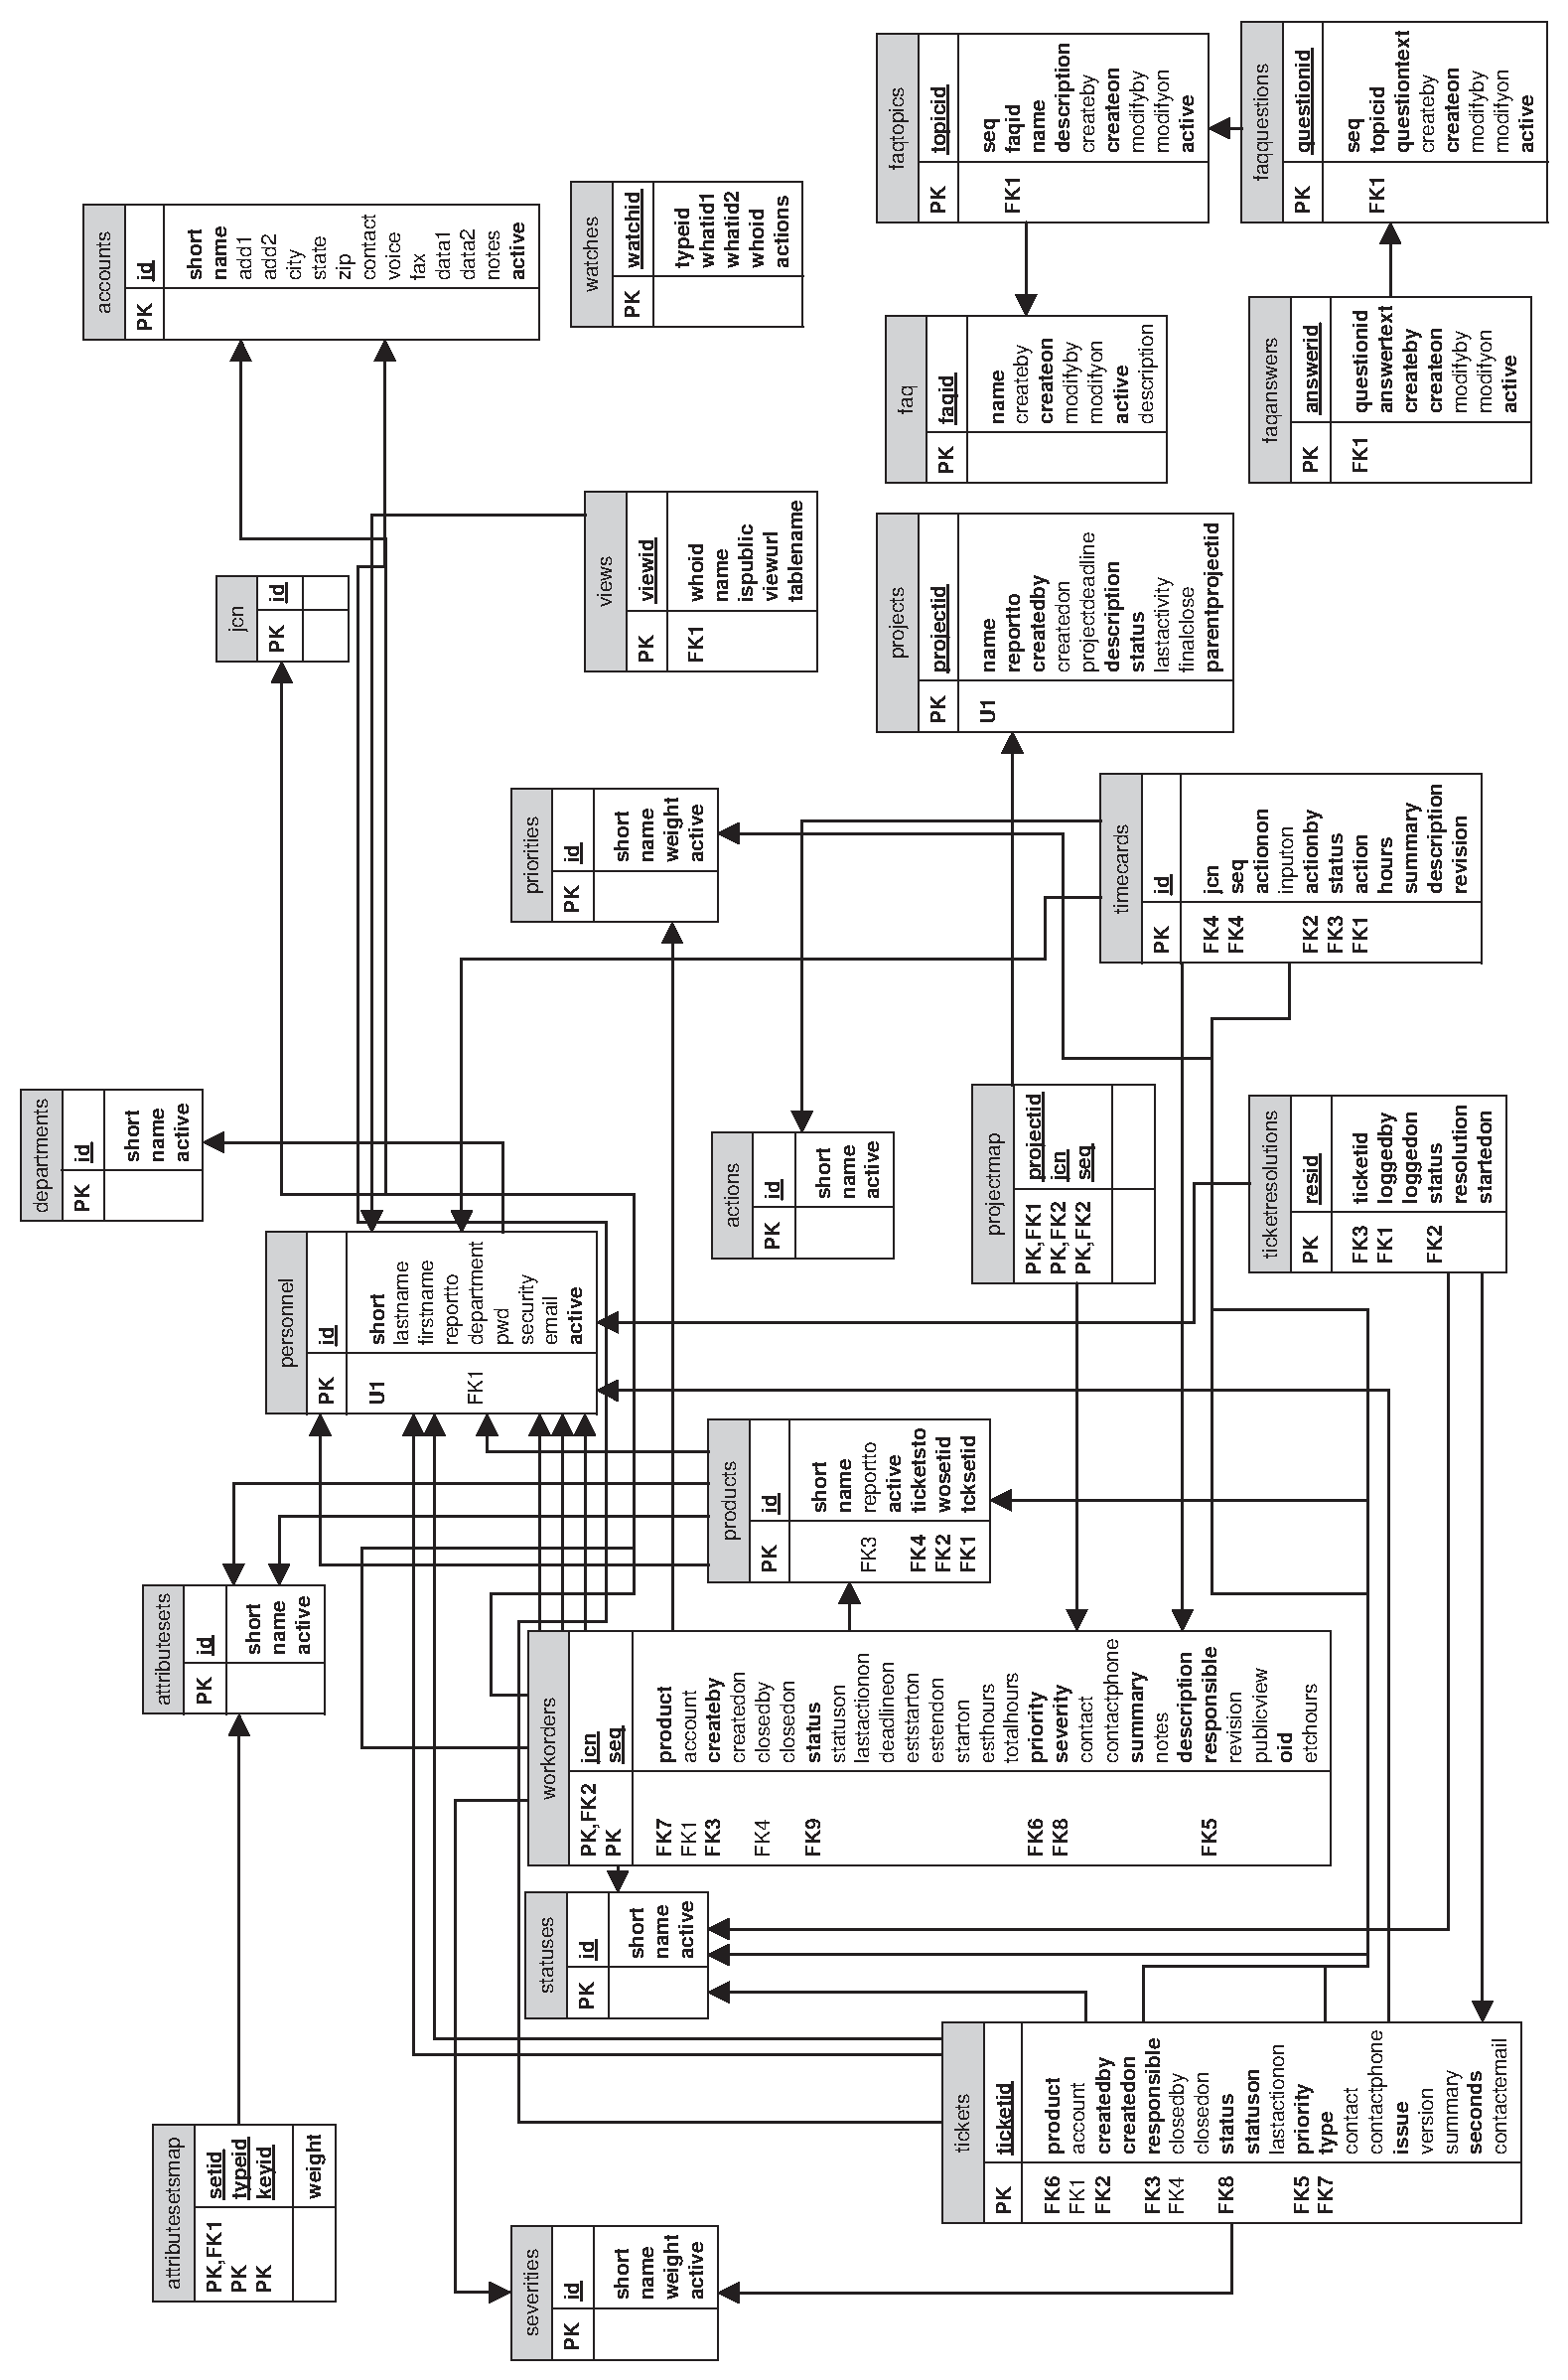
\includegraphics{DoubleChocoLatte.eps}} \par}
\vspace{0.3cm}


\section{TODO Feature List}


\subsection{\noindent Authentication}

\begin{itemize}
\item \noindent PAM Auth
\item \noindent Auto-Login via cookies
\item \noindent HTTP Auth
\item \noindent PHP4 Sessions (?)
\item \noindent Database sessions
\item \noindent LDAP Auth
\item \noindent Guest/public access
\item \noindent Authenticate via email address
\end{itemize}

\subsection{\noindent Work Orders}

\begin{itemize}
\item \noindent Search by department
\item \noindent Dependencies
\item \noindent Configurable fields (names, required, etc)
\item \noindent Scheduled E-mail of activity
\end{itemize}

\subsection{\noindent Project Management}

\begin{itemize}
\item \noindent Gantt Chart
\item \noindent Best fit scheduler
\item \noindent Tree view for projects
\item \noindent Change project status
\end{itemize}

\subsection{\noindent Tickets}

\begin{itemize}
\item \noindent Search by department
\item \noindent Configurable fields (names, required, etc)
\item \noindent Quality of service contract
\item \noindent Auto ticket priority upgrade
\item \noindent Allow multiple responsible
\item \noindent Aging ticket reminder
\item \noindent Queue support
\item \noindent Scheduled E-mail of activity
\end{itemize}

\subsection{\noindent Security}

\begin{itemize}
\item \noindent Roles and permissions
\item \noindent Customer access to system with account restriction
\item \noindent Verify authenticity of form submissions
\item \noindent Validate data submitted from forms on server side
\item \noindent Move attachment files outside of web dir and force client download
\end{itemize}

\subsection{\noindent E-mail Gateway}

\begin{itemize}
\item \noindent Work order submission/query
\item \noindent Ticket submission/query
\end{itemize}

\subsection{\noindent Reporting}

\begin{itemize}
\item \noindent More analysis and stats
\end{itemize}

\subsection{\noindent UI}

\begin{itemize}
\item \noindent Templatize menus so templates can be selected @ login
\end{itemize}

\subsection{\noindent NLS}

\begin{itemize}
\item \noindent Create db utility to maintain language files in str dir
\end{itemize}

\subsection{\noindent Accounts}

\begin{itemize}
\item \noindent Create client list w/many-to-many relationship
\item \noindent Associate products with account
\end{itemize}

\section{Contributors}

The following is a quick list of people who have contributed to DCL in one way
or another. If I forgot you, it's because I'm very disorganized ;-), but I'm
trying to get this complete. Just shoot me an email and what section you belong
in and I'll add you to the list.


\subsection{Core Developers}

\begin{itemize}
\item Michael Dean <mdean@users.sourceforge.net>
\end{itemize}

\subsection{Packagers}

\begin{itemize}
\item Debian - Ola Lundqvist
\end{itemize}

\subsection{Documentation}

\begin{itemize}
\item Michael Dean
\item Michael Brader
\end{itemize}

\subsection{Translations}

\begin{itemize}
\item English - Michael Dean :-)
\item Swedish - Ola Lundqvist
\item German - Herbert Mollien
\item French - Laurent Portefaix
\item Italian - Luca Pescatore, Angelo Addante
\end{itemize}

\subsection{Patches}

\begin{itemize}
\item Michael Brader
\item Brian Cooke
\item Urmet Janes
\item Ola Lundqvist
\item Jim Lieb
\item Evelyn Mitchell\end{itemize}

\end{document}
